\subsection{Use concepts and language that your user understands}

The key point is that the user must be able to understand what we are trying to transmit. We must create a fluid, 
easy interaction between the user and the representation of the data. Therefore we must speak with the language of 
the ordinary person, using common vocabulary, avoiding specialist jargon and communicating the objective in the simplest, 
clearest manner. This representation of information plays a fundamentally important role, enabling the user to absorb 
the meaning in a natural way.

\subsubsection*{Suggested strategies} 

Consider what type of representational format is most appropriate to the task. If it is not possible, we will provide de 
resources needed to help the user to understand and place the information in context. \\

We should stady which type of representation fits better to which kind of data,A graph may not necessarily be the 
clearest way to represent information.\\

We should take into account the target audience, and how we can most effectively transmit information to them. 
If we decide that a using graph is the best solution, we must consider carefully which type to use. For example, 
if we talk about samples and we want to know the density, we will lean towards a density graph, and if we look for the difference
between sexes, we will use a pie chart.

\subsubsection*{In the context of Aire Guru \ldots} 

The Aire Guru tool presents the information in the native language of the city, using simple vocabulary and a 
straightforward style. Colors and graphic resources are used as icons. In addition, a unified design structure to represent data has 
been used over the whole site, giving the user a consistent visualization experience. \\

One of the objectives is to represent pollution by areas of the city, which is why a map has been used - the 
obvious and familiar visual image of the different places in the city. This is a more legible format since the user
does not need to make a continous effort to place the data in each part of the city. The index shows an indicator with 
five levels represented by a color scale from the turquoise to red ("Good" "Fair" "Poor" "Bad" and "Unhealthy"). 
The color-coding is consistent with the colors which are used in official sources, thereby avoiding onfusion any 
user who might consult official sources.

\begin{figure}[ht]
    \centering
    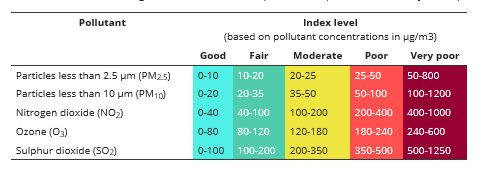
\includegraphics[width=12cm]{EAQI}
    \caption{EAQI Levels}
\end{figure}

These icons below are used to help the user have an immediate idea of the situation, since they are even more
decriptive and self-explanatory than just colors alone. Danger is, of course, almost universally indicated by 
the colour red, and is therefore used appropriately. However, no all cultures has the same perception about
the blue or green, missing what they indicate\\

\begin{figure}[ht]
    \centering
    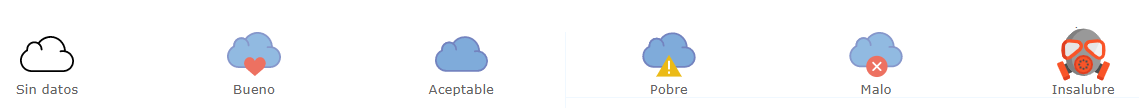
\includegraphics[width=10cm]{EAQI_Icons}
    \caption{Iconografica Aire Guru}
\end{figure}

For the graphs that show variations in time,  we have chosen line graphs as being most appropriate,
since they show the continuous evolution over a period of time. To represent the different components of the AQI, we chose a
graph of stacked bars, since it is easy to see what proportion of the total AQI is formed by which pollutant. \\

\begin{figure}[ht]
    \centering
    \subfigure[AQI Evolution]
        {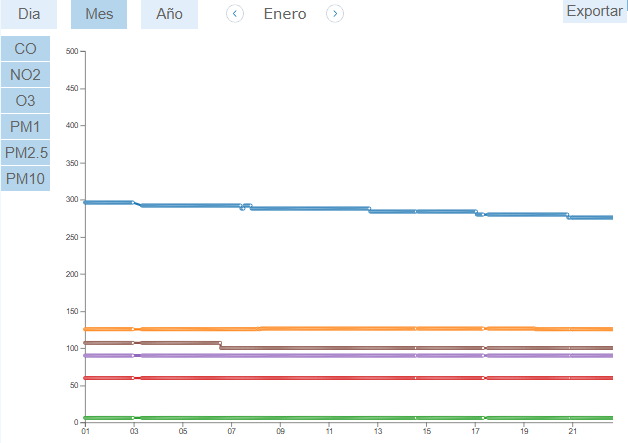
\includegraphics[width=5.75cm]{lineChart}}
        \hfill
    \subfigure [AQI components]
        {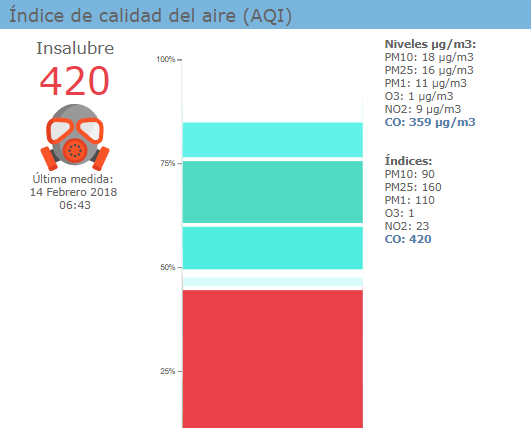
\includegraphics[width=5.25cm]{stakedBarChart}}
    \caption{Charts}
\end{figure}

In addition, to explain the concept of AQI and create an awarnes about the influence that air pollution has on us, Aire Guru includes it in the
glossary. This aids understanding of why air pollution should matter to us, with descriptions of the pollutants, medical complications, sources of contamination, the iconography used and
an explanation of what AQI is and how it is calculated. \\

\begin{itemize}
    \item The language used in the whole webtool is a common language, avoiding the use of difficult scientific terminology but providing clearly described information to understand the situation.
    \item The most appropriate graphs for each type of data have been researched and chosen.
    \item Some specific terms could not be substituted as "Air Quality Index".
    \item The tools necessary to understand the concept have been provided. The European standard of air quality has been used to
          represent the values and offer the user resources on the page for their comprehension in addition to external resources.
\end{itemize}